\begin{figure}[ht] 
 	\centering 
 	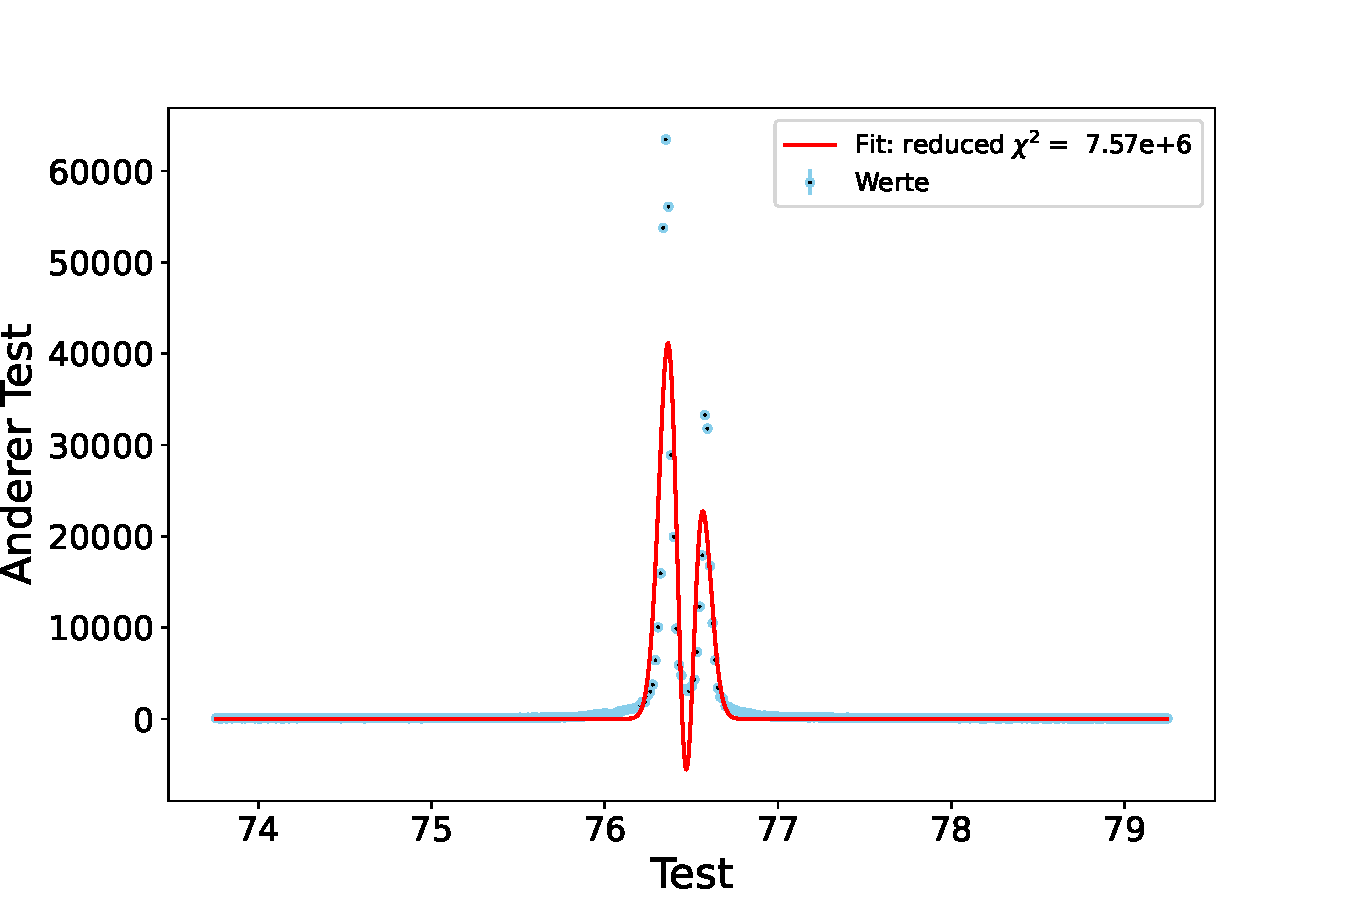
\includegraphics[width= 0.65 \textwidth]{Fits/data_test_Fit.pdf} 
	\caption{data_test, Fit} 
 	\label{fig:data_test, Fit} 
\end{figure}
 \\ 
\begin{table}[ht] 
\centering 
\caption{my-table} 
\label{tab:my-table}
\begin{tabular}{|l|c|}
\hline
Parameter Name	&	Wert \\ \hline
aamplitude	&	 3875.724 \pm  59.173\\ \hline
acenter	&	 76.356 \pm  0.000431\\ \hline
asigma	&	 0.0244 \pm  0.000431\\ \hline
bamplitude	&	 2088.403 \pm  62.302\\ \hline
bcenter	&	 76.584 \pm  0.000933\\ \hline
bsigma	&	 0.0271 \pm  0.000933\\ \hline
afwhm	&	 0.0575 \pm  0.00101\\ \hline
aheight	&	 63299.381 \pm  966.581\\ \hline
bfwhm	&	 0.0638 \pm  0.0022\\ \hline
bheight	&	 30769.148 \pm  918.037\\ \hline
\end{tabular} 
\end{table}